\chapter{Multicriteria Recommender Systems}
\graphicspath{{Chapter03/Figures/}}
\label{chap:multicriteria}

The traditional approach to the recommendation problem discussed in Section~\ref{soa:sec:recommender} could be considered somewhat limited, as users typically tends to judge items according to different criteria~\cite{Adomavicius2015}. For example, we can easily imagine to assign different ratings to a movie, expressing how much we liked the story, the acting, the direction, and the visual effects. Such multiple ratings could be exploited by a recommender system in order to identify more effectively which items should be suggested. For this reason, different authors started to propose multicriteria recommender systems, namely methods capable of suggesting items by relying on ratings provided over different criteria instead of a single one~\cite{Adomavicius2005,Manouselis2007}.

In this chapter, we investigate the state of the art in the field of multicriteria recommender systems. We follow the systematic literature review protocol proposed by Kitchenham \& Charters~\cite{Kitchenham07}, in order to enable other researchers to easily verify and reproduce our work. We consider nine different research questions that encompass various aspects of the reviewed studies.

In particular, we analyze the most important problems that multicriteria recommenders aim to address, as well as the exploited recommendation approaches, according to the taxonomy created by Burke~\cite{Burke2007}. We also describe the different machine learning and data mining techniques typically included in a multicriteria recommender and we identify which methods are frequently utilized in each recommendation phase, thus we try to describe the structure of an ideal multicriteria RS. We quantitatively measure the domains that are the most appropriate ones for such systems and we review how the proposed algorithms have been evaluated with respect to the experimental settings, the metrics, and the exploited datasets. Finally, we describe the most promising directions for future works that are mentioned in the reviewed studies.

We considered a total number of 93 studies, published from 2003 to 2018, to perform this systematic literature review. To the best of our knowledge, this is the first review conducted in the field of multicriteria recommender systems that follows a standardized and repeatable protocol. We aim that our study could be useful to other researchers working in this area, especially for better identifying possible approaches and future trends.

The remainder of this chapter is structured as follows. In Section~\ref{mcr:sec:methodology}, we detail the protocol that we followed for conducting the review. Then, we present the quantitative results in Section~\ref{mcr:sec:results} and we provide a possible interpretation of the outcomes of the review in Section~\ref{mcr:sec:discussion}. Finally, we conclude this chapter with Section~\ref{mcr:sec:conclusions}, while, in Appendix~\ref{chap:studies-slr}, we report the list of selected studies.

\section{Methodology}
\label{mcr:sec:methodology}

We decided to perform this review according to the guidelines designed by Kitchenham \& Charters for Systematic Literature Reviews (SLR) in the field of Software Engineering~\cite{Kitchenham07}. This method guarantees that the outcome of the review is verifiable and repeatable by other researches. The protocol, which is graphically illustrated in Figure~\ref{mcr:fig:protocol}, was developed by the author of this dissertation.

\begin{figure}
\centering
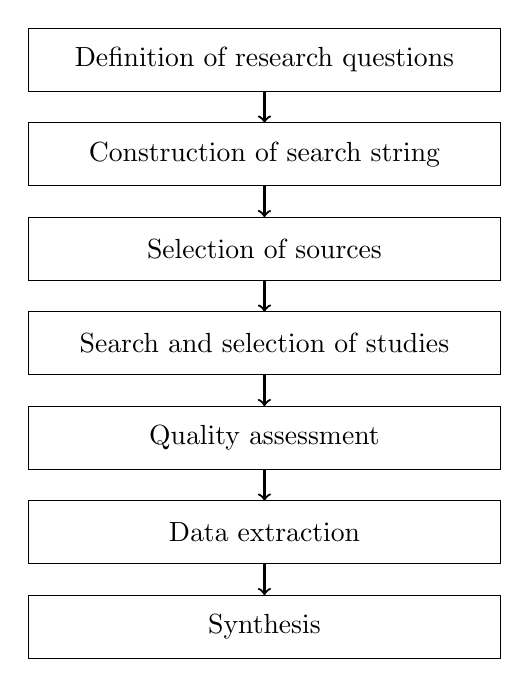
\begin{tikzpicture}
\draw (0,0) rectangle (6,-0.8);
\draw (3,-0.4) node {Definition of research questions};
\draw[thick,->] (3,-0.8) -- (3,-1.2);
\draw (0,-1.2) rectangle (6,-2);
\draw (3,-1.6) node {Construction of search string};
\draw[thick,->] (3,-2) -- (3,-2.4);
\draw (0,-2.4) rectangle (6,-3.2);
\draw (3,-2.8) node {Selection of sources};
\draw[thick,->] (3,-3.2) -- (3,-3.6);
\draw (0,-3.6) rectangle (6,-4.4);
\draw (3,-4) node {Search and selection of studies};
\draw[thick,->] (3,-4.4) -- (3,-4.8);
\draw (0,-4.8) rectangle (6,-5.6);
\draw (3,-5.2) node {Quality assessment};
\draw[thick,->] (3,-5.6) -- (3,-6);
\draw (0,-6) rectangle (6,-6.8);
\draw (3,-6.4) node {Data extraction};
\draw[thick,->] (3,-6.8) -- (3,-7.2);
\draw (0,-7.2) rectangle (6,-8);
\draw (3,-7.6) node {Synthesis};
\end{tikzpicture}
\caption[Systematic literature review protocol]{The systematic literature review protocol designed following the guidelines by Kitchenham \& Charters~\cite{Kitchenham07}.}
\label{mcr:fig:protocol}
\end{figure}

\subsection{Research Questions and Search String}
\label{mcr:sec:questions}

The purpose of this systematic literature review is to identify the studies describing multicriteria recommender systems and to understand the motivations behind their usage, the techniques employed, the experimental protocols used to validate them, and the related research challenges. For these reasons, we defined the following research questions.

\begin{description}
\item[RQ1.1\label{mcr:itm:rq1}] What are the most relevant studies addressing multicriteria RSs?
\item[RQ1.2\label{mcr:itm:rq2}] What are the most challenging problems faced by researchers?
\item[RQ1.3\label{mcr:itm:rq3}] What are the approaches used by multicriteria recommenders?
\item[RQ1.4\label{mcr:itm:rq4}] Which techniques and methods have been proposed?
\item[RQ1.5\label{mcr:itm:rq5}] In which domains multicriteria recommender systems are applied?
\item[RQ1.6\label{mcr:itm:rq6}] Which protocols and frameworks are used for their evaluation?
\item[RQ1.7\label{mcr:itm:rq7}] Which metrics are considered during their evaluation?
\item[RQ1.8\label{mcr:itm:rq8}] Which datasets are used for testing the algorithms?
\item[RQ1.9\label{mcr:itm:rq9}] What are the most promising directions for future works?
\end{description}

In order to retrieve the studies related to multicriteria recommender systems, we defined the following preliminary set of keywords: \{Multicriteria, Recommender System\}. This initial set was expanded to include alternative spellings and we defined the search string used to query the digital sources as follows.

\begin{lstlisting}
(multicriteria OR "multi criteria" OR "multi-criteria") AND ("recommender system" OR "recommendation system")
\end{lstlisting}

We selected six scientific digital libraries that contain primary studies related to the field of computer science, as detailed in Table~\ref{mcr:tab:sources}. Other more general sources, like Google Scholar, were not included because they usually index studies already available in the primary sources.

\begin{table}
\centering
\begin{tabular}{@{}ll@{}}
\toprule
Source               & URL                                 \\ \midrule
ACM Digital Library  & \url{https://dl.acm.org}            \\
IEEE Xplore          & \url{http://ieeexplore.ieee.org}    \\
ISI Web of Knowledge & \url{http://www.webofknowledge.com} \\
ScienceDirect        & \url{https://www.sciencedirect.com} \\
Scopus               & \url{https://www.scopus.com}        \\
Springer Link        & \url{https://link.springer.com}     \\ \bottomrule
\end{tabular}
\caption[Digital libraries considered]{The digital libraries considered during the search process.}
\label{mcr:tab:sources}
\end{table}

\subsection{Selection Process}

The selection process \added{was performed} during January 2019. We inserted the search query in the search field of the digital libraries selected as sources for the review and we retrieved all the studies identified by the respective search engines. \added{Because of the high number of false positive results, we decided to limit our search to the title, abstract, and keywords with IEEE Xplore, ISI Web of Knowledge, and Scopus.} The preliminary set \added{initially contained} $1256$ studies. We checked their titles and authors in order to discover possible duplicates: after having removed duplicated results, the preliminary set \added{was reduced} to $950$ studies.

Furthermore, for objectively identifying the studies to include in the review, we defined a set of inclusion and exclusion criteria, which are summarized in Table~\ref{mcr:tab:criteria}. We first applied the criteria in a coarse selection phase by only considering their abstracts and we obtained a list of $301$ papers. Then, we analyzed again the available studies in a detailed selection phase by reading relevant portions of their content. We finally selected $93$ studies as part of this literature review, as summarized in Table~\ref{mcr:tab:numbers}. The full list, \added{sorted by source, year of publication and author,} is available in Appendix~\ref{chap:studies-slr}.

\begin{table}
\centering
\begin{tabular}{@{}ll@{}}
\toprule
Code & Inclusion criteria \\ \midrule
IC1 & Papers describing multicriteria recommender systems \\
IC2 & Papers published in conferences and journals \\
IC3 & Papers written in English language \\ \midrule
Code & Exclusion criteria \\ \midrule
EC1 & Papers not addressing recommender systems \\
EC2 & Papers addressing RSs without multicriteria ratings \\
EC3 & Papers that report only abstracts or posters \\
EC4 & Papers that describe a planned research\footnotemark \\
EC5 & Grey literature and book chapters \\ \bottomrule
\end{tabular}
\caption[Inclusion and exclusion criteria]{The inclusion and exclusion criteria.}
\label{mcr:tab:criteria}
\end{table}
\footnotetext{\added{We defined a planned research as a study that only contains a high level description of the proposed methodology, without the details necessary to implement it.}}

\begin{table}
\centering
\begin{tabular}{@{}llll@{}}
\toprule
Source               & Search & Coarse & Detailed \\ \midrule
ACM Digital Library  & 27     & 24     & 11       \\
IEEE Xplore          & 38     & 36     & 15       \\
ISI Web of Knowledge & 31     & 25     & 6        \\
ScienceDirect        & 344    & 81     & 19       \\
Scopus               & 118    & 62     & 24       \\
Springer Link        & 392    & 73     & 18       \\ \midrule
Total                & 950    & 301    & 93       \\ \bottomrule
\end{tabular}
\caption[Studies per selection step]{The number of studies after each selection step.}
\label{mcr:tab:numbers}
\end{table}

\subsection{Quality Assessment}

For objectively assessing the quality of the studies selected as part of this review, we defined eight quality questions, as listed in Table~\ref{mcr:tab:quality}. It is possible to assign to each question the scores of $0$, $0.5$, and $1$, that correspond, respectively, to the answers \emph{Yes}, \emph{Partly}, and \emph{No}. During the quality assessment phase, we provided an answer to each question for all studies included in the review.
 
\begin{table}
\centering
\begin{tabular}{@{}ll@{}}
\toprule
Code & Quality question \\ \midrule
QQ1 & Did the study clearly describe the problems that it is addressing? \\
QQ2 & Did the study review the related work for the problem? \\
QQ3 & Did the study compare its approach with possible alternatives? \\
QQ4 & Did the study describe the components of the proposed RS? \\
QQ5 & Did the study provide an empirical evaluation of the solution? \\
QQ6 & Did the study present a clear statement of the findings? \\
QQ7 & Did the study analyze the application scenarios of the RS? \\
QQ8 & Did the study recommend any further research activity? \\ \bottomrule
\end{tabular}
\caption[Quality questions]{The quality questions.}
\label{mcr:tab:quality}
\end{table}

\subsection{Data Extraction}

We carefully read multiple times the primary studies \added{that are} selected as part of this review. During this phase, we identified the data available in the works useful for providing an answer to the research questions introduced in Section~\ref{mcr:sec:questions}. More in details, we looked for the information listed in Table~\ref{mcr:tab:form}. This process was supported by the data analysis software tool NVivo.\footnote{\url{https://www.qsrinternational.com/nvivo}} \added{We relied on this tool to minimize the manual effort required for applying the methodology described in Section~\ref{mcr:sec:synthesis}.}

\begin{table}
\centering
\begin{tabular}{@{}lll@{}}
\toprule
Field & Description & RQ  \\ \midrule
Code & An internal identifier of the study & - \\
Title & - & \ref{mcr:itm:rq1} \\
Authors & - & - \\
Publication year & - & \ref{mcr:itm:rq1} \\
Publication name & - & - \\
Source & The digital library that contains the study & - \\
Type & Conference or journal & - \\
DOI & - & - \\
Research problem & The problem that the study tries to address & \ref{mcr:itm:rq2} \\
Contribution & The description of the proposed method & \ref{mcr:itm:rq3} \\
Implementation & How the method was implemented & \ref{mcr:itm:rq4} \\
Domain & The domain of the recommended items & \ref{mcr:itm:rq5} \\
Evaluation protocol & The protocol used to evaluate the method & \ref{mcr:itm:rq6} \\
Evaluation metric & The metric used to compare the RS & \ref{mcr:itm:rq7} \\
Dataset & The dataset used to execute the evaluation & \ref{mcr:itm:rq8} \\
Limitation & The limitations of the proposed method & \ref{mcr:itm:rq9} \\
Future work & The suggestions for future works & \ref{mcr:itm:rq9} \\
Quality score & - & - \\ \bottomrule
\end{tabular}
\caption[Data extraction form]{The data extraction form.}
\label{mcr:tab:form}
\end{table}

\subsection{Synthesis}
\label{mcr:sec:synthesis}

We synthesized the results of our review following the Cruzes \& Dyba methodology~\cite{Cruzes2011} for combining and comparing the results of the primary studies that we considered. While reading the selected studies, we associated relevant portions of their text with codes. A code is a label applied to text segments that discuss the same theoretical or descriptive idea and that is used to aggregate in an organic way the data that we are analyzing. We initially defined some general codes associated with the research questions. Then, we created more specialized sub-codes related to the content of the studies, thus following an integrated approach that combines both inductive and deductive methods and that is considered the most appropriate one for a systematic review~\cite{Cruzes2011}. We subsequently aggregated the codes in themes, and we mapped these themes back to the original research questions. The outcomes of this last phase are reported in Section~\ref{mcr:sec:results}, grouped by research question.

\section{Results}
\label{mcr:sec:results}

In this section, we highlight the findings of our systematic literature review regarding multicriteria recommender systems, according to the research questions introduced in Section~\ref{mcr:sec:questions}. These results will be further discussed in Section~\ref{mcr:sec:discussion}.

\subsection{Included Studies}
\label{mcr:sec:included}

The main purpose of \ref{mcr:itm:rq1} is to identify the studies related to the topic of multicriteria recommender systems to be included in this review. Following the protocol detailed in Section~\ref{mcr:sec:methodology}, we identified a total number of $93$ studies. These works have been presented during conferences or they have been published in scientific journals in a period of time from 2003 to 2018. In Figure~\ref{mcr:fig:study-per-year}, we detail the number of studies per year and per venue. It is possible to observe an increasing amount of studies published in the last years.\footnote{Please note that the results for the year 2019 are not available, as the selection was performed in January 2019.}

We exploited the questions listed in Table~\ref{mcr:tab:quality} to assess the quality of the works included in this review. In Figure~\ref{mcr:fig:quality-per-type}, we report the quality scores according to the publication venue. As expected, journal papers obtained, in general, higher scores with respect to conference papers. Furthermore, Figure~\ref{mcr:fig:quality-per-question} contains the average quality scores for each quality question. It is possible to observe that the highest scores are associated with QQ1 (\emph{Did the study clearly describe the problems that it is addressing}?), while the lowest ones with QQ8 (\emph{Did the study recommend any further research activity?}).

\begin{figure}
\centering
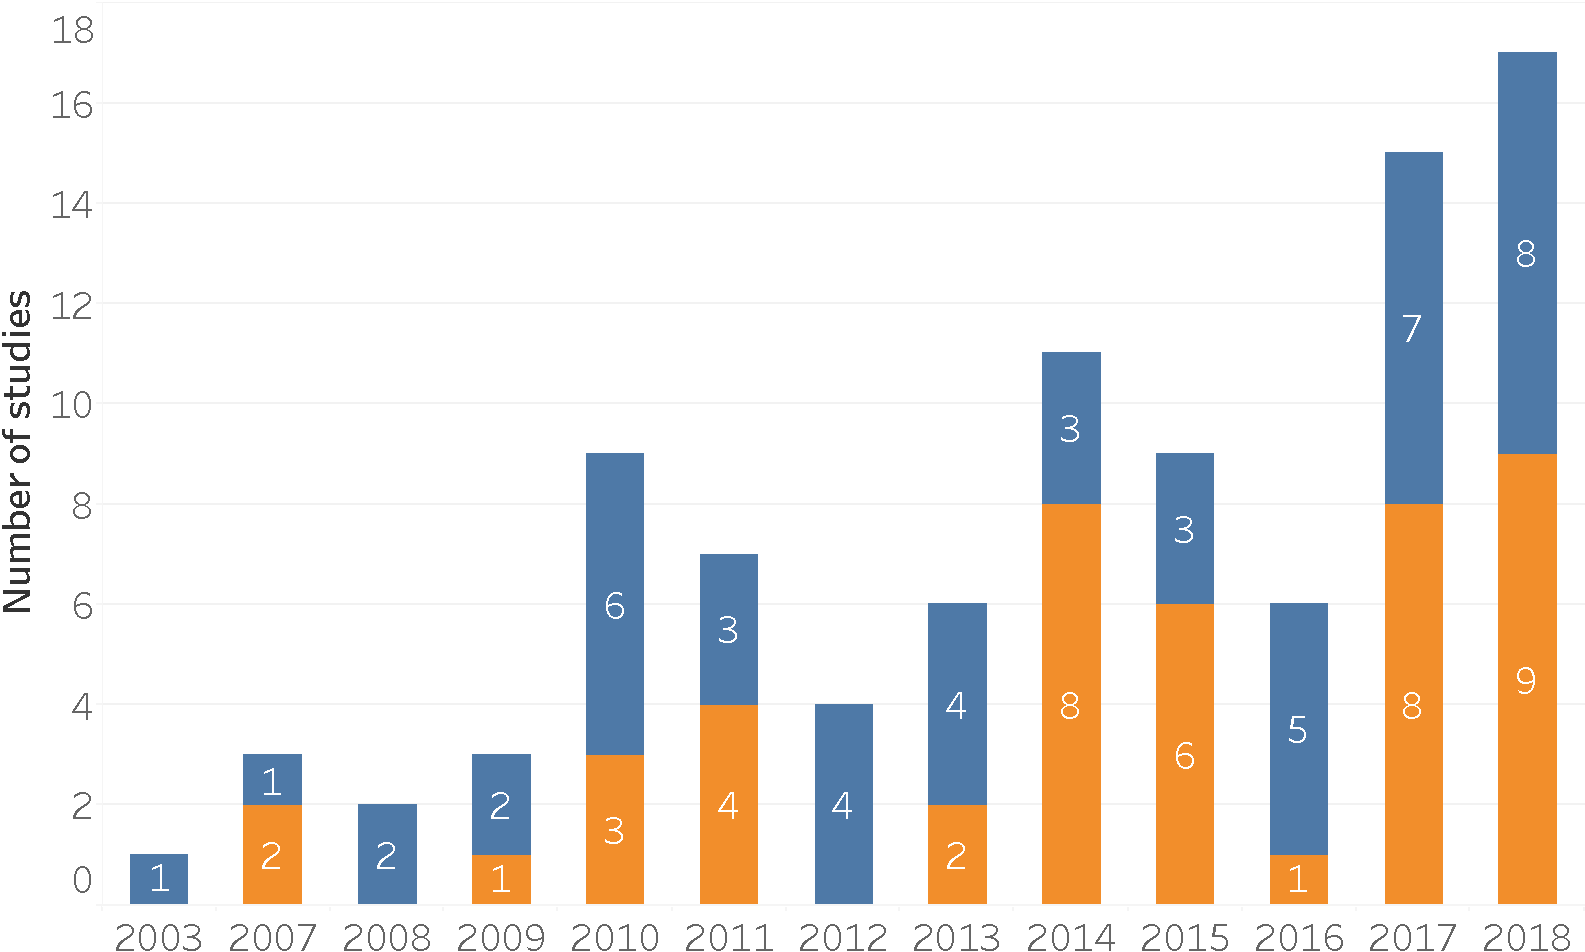
\includegraphics[width=\textwidth]{study_per_year}
\caption[Studies per year of publication]{This stacked barplot represents the number of included studies per year of publication. Blue studies have been presented in a conference, while orange studies have been published in a journal.}
\label{mcr:fig:study-per-year}
\end{figure}

\begin{figure}
\centering
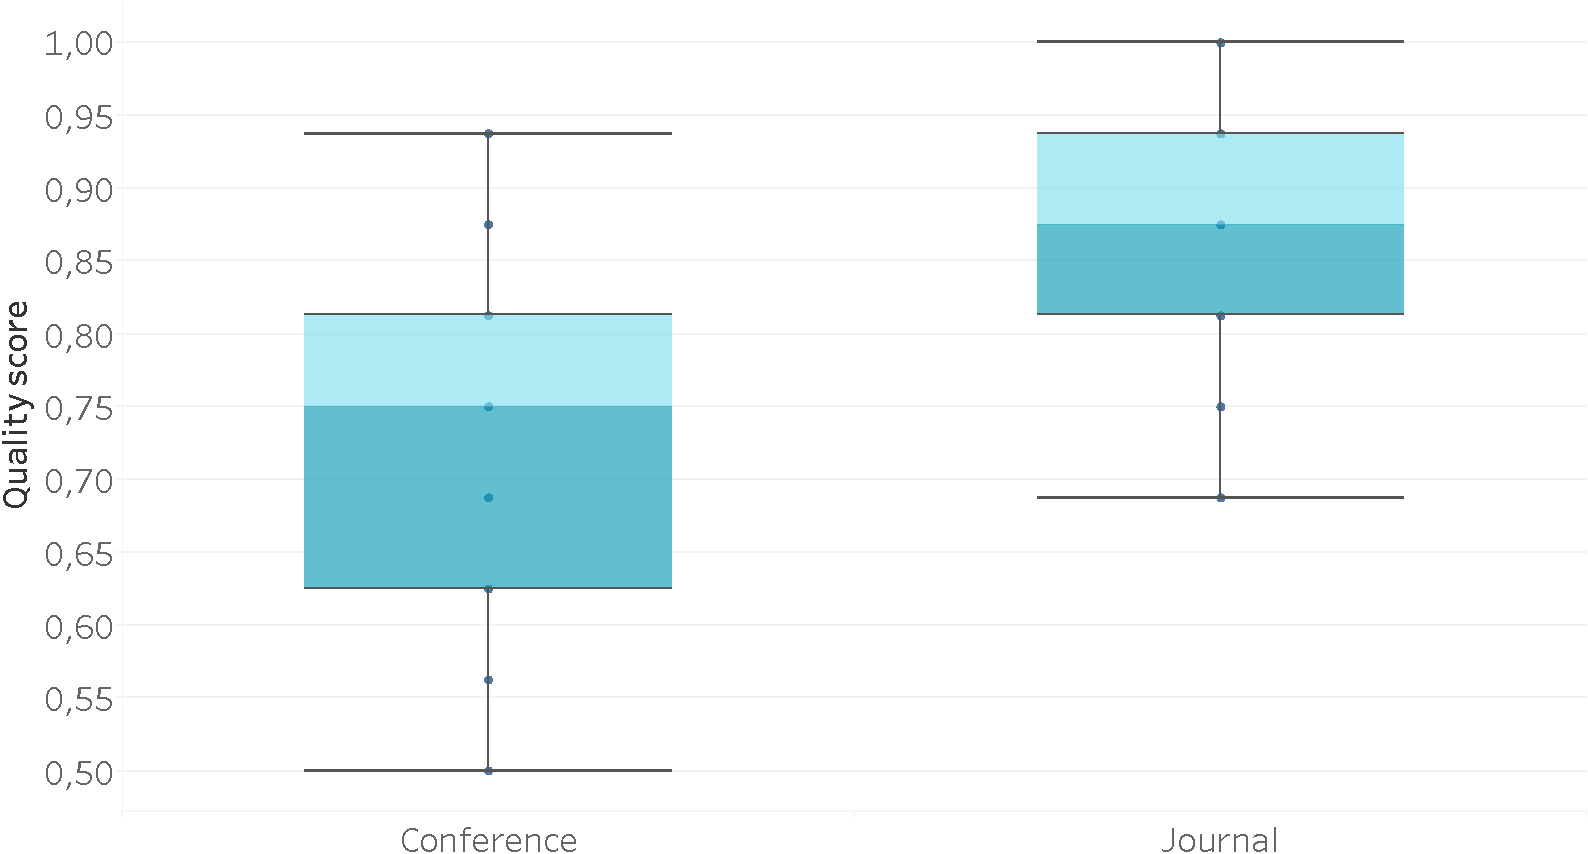
\includegraphics[width=\textwidth]{quality_per_type}
\caption[Quality scores per publication type]{This boxplot represents the distribution of quality scores per publication type. Studies published in journals have higher quality scores.}
\label{mcr:fig:quality-per-type}
\end{figure}

\begin{figure}
\centering
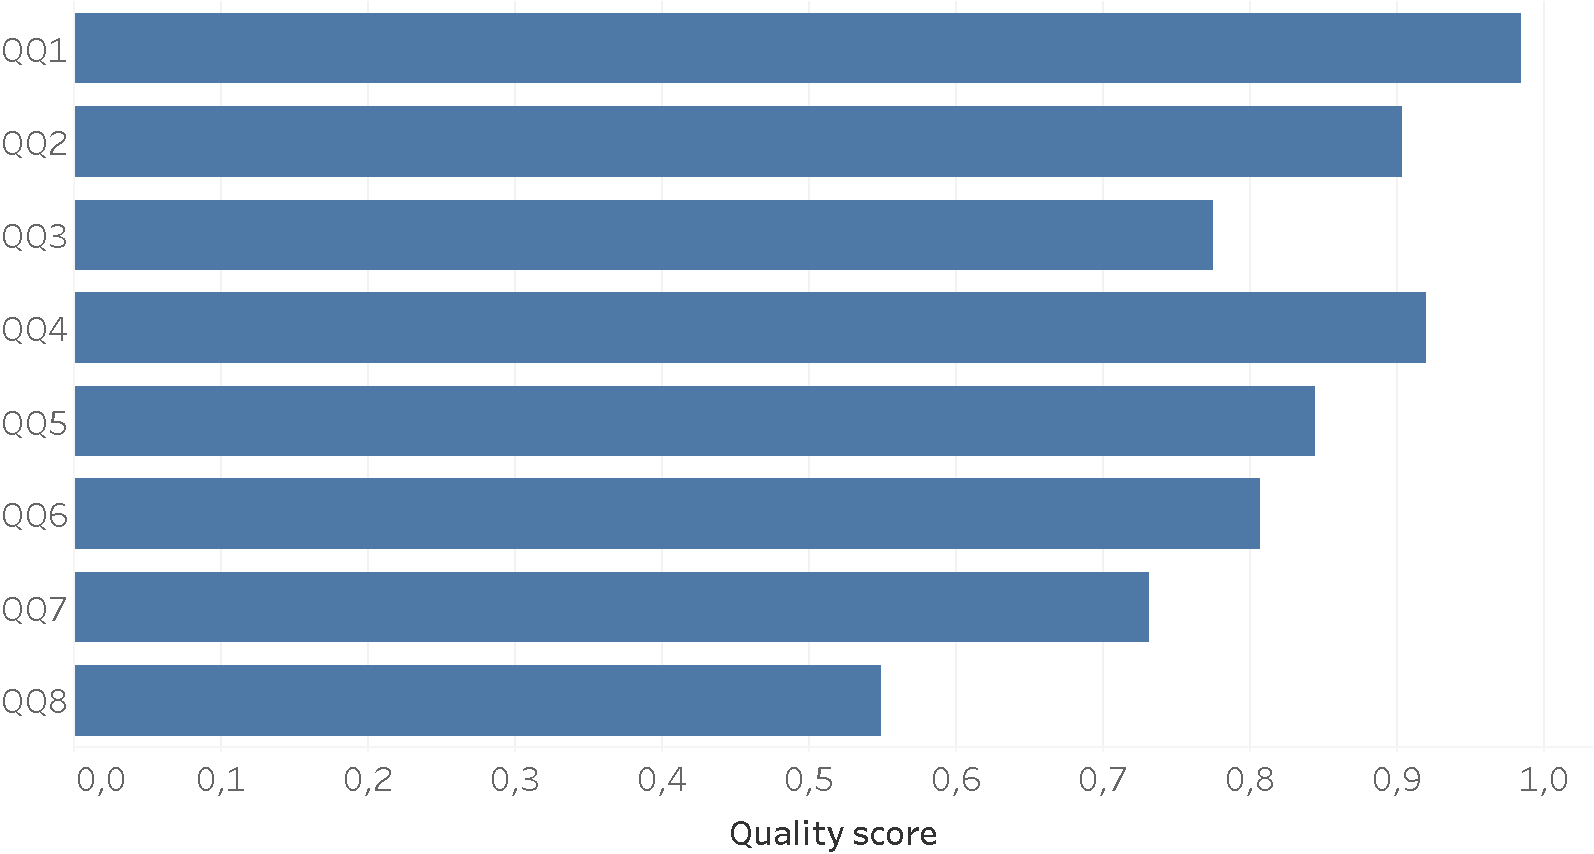
\includegraphics[width=\textwidth]{quality_per_question}
\caption[Quality score per quality question]{This barplot represents the average quality score per quality question. The lowest quality score is associated with the description of future works.}
\label{mcr:fig:quality-per-question}
\end{figure}

\subsection{Research Problems}
\label{mcr:sec:problems}

In this section, we describe the main problems and challenges that multicriteria recommender systems aim to address and, thus, we provide an answer to \ref{mcr:itm:rq2}. In total, we identified 10 different categories of problems that are mentioned in the reviewed studies. The number of studies for each category is summarized in Figure~\ref{mcr:fig:study-per-problem}. It is important to observe that a single study may \added{analyze} different problems at the same time.

\subsubsection{Data Sparsity}

Data sparsity is the most frequent problem in this field and it is caused by the fact that users provide ratings for a limited number of items or criteria. While this is a well documented common issue of recommender systems, multicriteria user-item matrices may be even sparser, as they require more effort and time from the users of the system. In order to address this problem, several solutions are proposed in the reviewed studies. For example, the authors of \pref{slr:Jannach2012} suggest to combine the multicriteria ratings using two different regression functions, one for the items and one for the users. The ratings estimated by the regression functions are then combined in order to minimize the prediction error. In \pref{slr:Samatthiyadikun2013}, a Bayesian latent model for multicriteria recommenders is exploited along with a support vector regression learner in order to mitigate the data sparsity problem. Another possible solution, as suggested in \pref{slr:Premchaiswadi2013}, is represented by dimensionality reduction techniques, which can be used to obtain a more compact representation of each user. Finally, it is possible to integrate the available ratings with an external ontology~\pref{slr:Liu2010} or with a trust-based model~\pref{slr:Goswami2017}. The data sparsity problem was identified in a total number of 22 studies.

\subsubsection{Criteria Weights}
\label{mcr:sec:criteria-weights}

In order to provide accurate suggestions, it is of paramount importance being able to discover the relationships among the different criteria and to identify the most relevant ones for the target user. A wide range of possible solutions is available in the analyzed studies. For instance, the authors of \pref{slr:Sreepada2017} identify the most important criteria for a user exploiting a statistical technique based on the average ratings of each item. Other studies analyze several machine learning methods. In \pref{slr:Zheng2017}, the author proposes to consider \emph{chains} of criteria instead of exploiting all criteria together: the rating on each criterion is estimated considering the previous predictions as context information. In \pref{slr:Choudhary2017}, the optimal weights are learned using particle swarm optimization, while in \pref{slr:Ding2018b} an artificial neural network is exploited for this purpose. Another popular solution is represented by decision making methods. As an example, in \pref{slr:Song2018} users are asked to perform pair-wise comparisons of the available criteria. The problem of selecting proper criteria weights was explicitly mentioned in 17 studies.

\subsubsection{\added{Personalization}}
\label{mcr:sec:personalization}

Any recommender system should be capable of suggesting items that match the preferences of the target user. The possibility of exploiting multiple ratings for each item is often considered an effective way of increasing the accuracy of the recommendations, for example this fact is mentioned in \pref{slr:Shambour2010} and \pref{slr:Mikeli2015}. It is also important being able to understand what are the most relevant criteria for each user, as suggested by the authors of \pref{slr:Sreepada2017}. On the other hand, it is essential to avoid including criteria that are redundant, as this may negatively affect the performance of the system~\pref{slr:Yin2009}. In \pref{slr:Castillo2018}, a multicriteria recommender system is combined with a content-based approach in order to generate better suggestions, while the authors of \pref{slr:Tallapally2018} propose to increase the accuracy of the recommendations using a deep learning technique called Stacked Autoencoders. In general, this problem was explicitly considered by 15 studies.

\subsubsection{Data Noise}
\label{mcr:sec:data-noise}

The presence of noise in data is typically related to the fact that users may provide ratings that are biased or even dishonest. For example, users may not understand the meaning of each criterion \added{and} may find difficult to express their preferences on a numerical scale, or may be bored by the request of assigning many ratings to a single item. In \pref{slr:Kant2017}, fuzzy logic techniques are exploited in order to \added{address} the uncertainty of user preferences, while in \pref{slr:Goswami2017} such techniques are combined with a trust-based model. The authors of \pref{slr:Jannach2012} propose to mitigate this problem by performing feature selection in a pre-processing step, where the most relevant criteria of a certain dataset are identified. Another possible solution to this problem is represented by the idea of considering the numerical differences between ratings instead of their absolute values in the recommendation process~\pref{slr:Mikeli2015}. Data noise was addressed by 14 studies.

\subsubsection{Cold-start}
\label{mcr:sec:cold-start}

The cold-start problem is a well-known issue in the field of recommender systems based on collaborative filtering approaches. It can be defined as the impossibility of creating reliable suggestions due to the lack of data regarding a new user or a new item. The authors of \pref{slr:Palanivel2011} aim to solve it by providing non-personalized recommendations to new users and exploiting content-based features when a new item is added to the system. A different approach is represented by the elicitation of user preferences using decision making techniques and multicriteria ratings \pref{slr:Hdioud2014}. In \pref{slr:Akcayol2018}, a multicriteria implicit feedback method based on user behavior analysis is discussed, while the authors of \pref{slr:Shambour2010} propose to tackle this issue with a trust-based model. As a last example, a knowledge-based method that is immune to the cold-start problem is illustrated in \pref{slr:Niknafs2008}. Cold-start was considered a research issue in 14 studies.  

\subsubsection{Scalability}
\label{mcr:sec:scalability}

Scalability is a general problem of collaborative filtering recommender systems, especially \added{for} the ones developed in an academic context \added{as proof-of-concept}. Because many multicriteria recommenders require multiple runs of such algorithms, it is reasonable to suppose that scalability issues are even more widespread. For example, this issue is discussed by the authors of \pref{slr:Wijayanto2016}, who describe a multicriteria recommender that exploits a distributed architecture based on Apache Spark. In \pref{slr:Mikeli2015}, a clustering algorithm is applied for creating groups of similar users that can be used to compute predictions in a scalable way. A popular dimensionality reduction technique discussed by \pref{slr:Bokde2015} and \pref{slr:Nilashi2014b} is the higher order single value decomposition. In total, 12 studies considered the scalability problem.

\subsubsection{User's Effort}

As multicriteria recommenders usually require many ratings for each user and item pair, explicit elicitation methods are intrusive and may waste the user's effort and time. For this reason, the authors of \pref{slr:Palanivel2010} and of \pref{slr:Nunez-Valdez2018} propose a multicriteria recommender based only on implicit feedback. Another possible solution is described in \pref{slr:Premchaiswadi2013}, where \added{their} authors develop a hybrid profiling framework for reusing traditional ratings with multicriteria recommenders. A similar approach to this problem is presented in \pref{slr:Castillo2018}, where multicriteria ratings are computed starting from single ratings and content-based information. This problem was discussed by 11 studies.

\subsubsection{Other Research Problems}

Other research problems are mentioned in a more limited number of studies. In particular, 4 studies analyzed the issues related to the selection of a proper similarity metric in the context of multidimensional neighborhood-based collaborative filtering, while 3 studies reported the challenges related to the execution of a reliable evaluation protocol. Finally, 3 more recent studies mentioned the problem of fairness in the selection of the recommended items, both with respect to the unique peculiarities of the users and to the characteristics of the catalog.

\begin{figure}
\centering
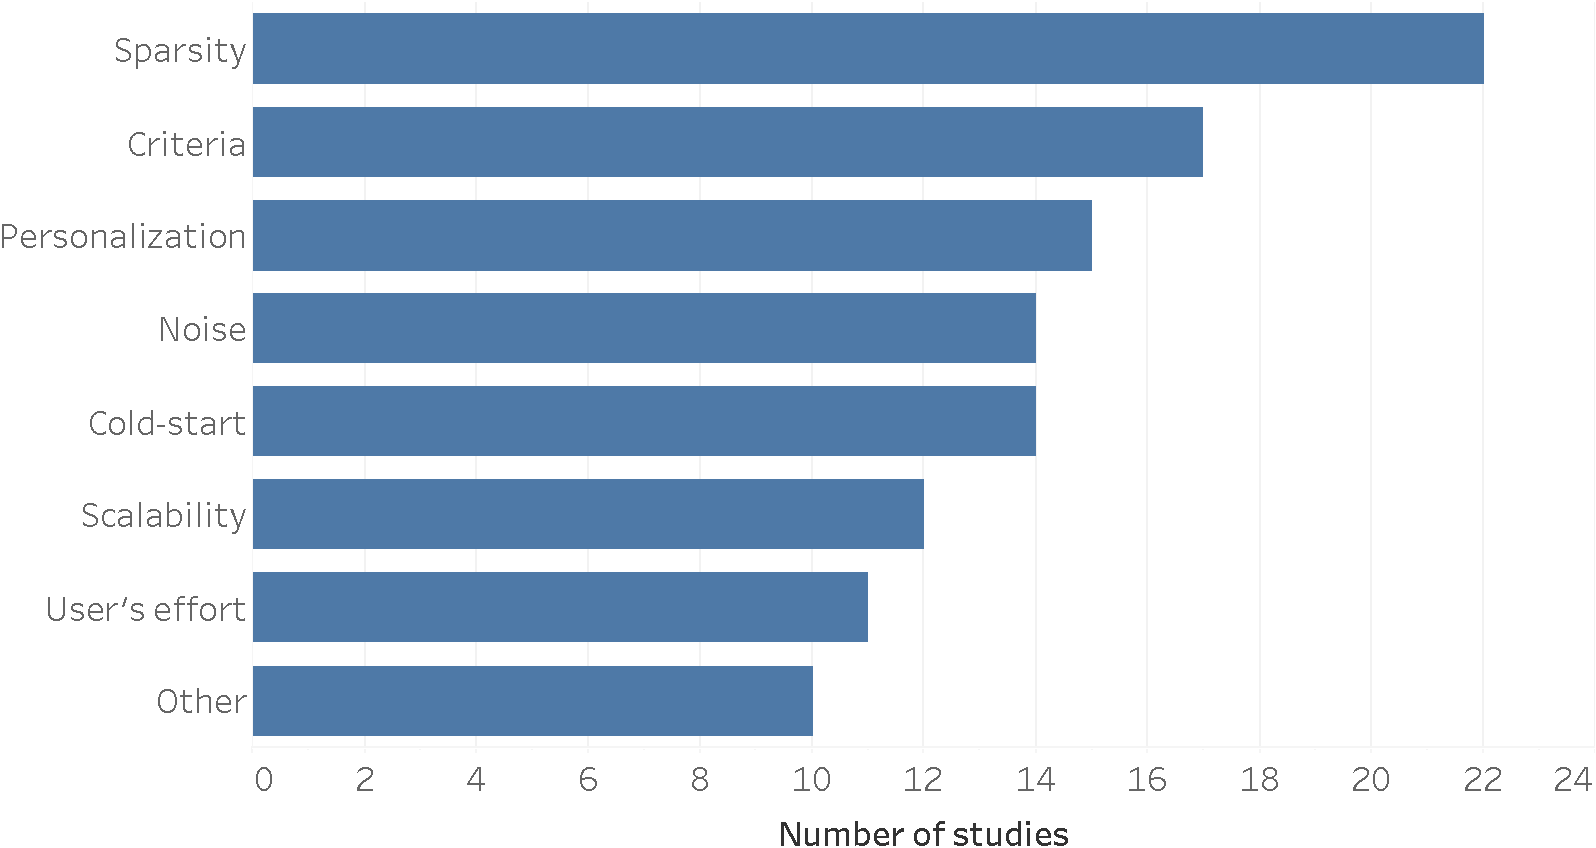
\includegraphics[width=\textwidth]{problem_per_study}
\caption[Studies per research problem]{This barplot represents the number of studies per research problem.}
\label{mcr:fig:study-per-problem}
\end{figure}

\subsection{Recommendation Approaches}
\label{mcr:sec:approaches}

In order to provide an answer to \ref{mcr:itm:rq3}, we analyzed the studies included in this systematic literature review and we classified them according to the taxonomy provided by Burke~\cite{Burke2007}. This taxonomy has become a widespread way of characterizing different recommendation approaches. However, we decided not to consider hybrid recommender systems, as almost all multicriteria recommenders would fall in this category. For this reason, if a study combines multiple approaches, it will be included in all the categories of the different methods that are mentioned in the study. We summarize the number of available studies for each recommendation approach in Table~\ref{mcr:tab:study-per-approach}.

\subsubsection{Collaborative Filtering}

Collaborative filtering is the most popular recommendation technique described in the reviewed literature. In a traditional recommender system, the users whose rating behaviour is similar to the one of the target user are exploited for selecting the items to be suggested. In a multicriteria recommender, a popular approach consists in applying collaborative filtering algorithms on the available criteria and then combining the results in a global estimated rating, like in \pref{slr:Hwang2010} and \pref{slr:Manouselis2007}. An alternative to the user-based approach is represented by the item-based collaborative filtering, where the similarity is computed among the items, as discussed, for example, in \pref{slr:Bilge2014}. \added{The authors of} \pref{slr:Jannach2012} and \pref{slr:Kermany2017} describe how to combine user-based and item-based models in a comprehensive approach. Collaborative filtering may also be implemented with a model-based approach, for instance matrix factorization (e.g., in \pref{slr:Asawarangsee2016} and \pref{slr:Majumder2017}). In general, this technique may be combined with other methods, like content-based approaches~\pref{slr:Zarrinkalam2012}, clustering~\pref{slr:Mikeli2015}, and fuzzy logic~\pref{slr:Palanivel2011}. In total, collaborative filtering was exploited by 82 studies.

\subsubsection{Content-based}

A content-based recommender system considers the previous preferences of a user in order to build a profile and to select items with similar characteristics. For example, the authors of \pref{slr:Naak2009} describe a recommender system of research papers that relies on content-based and multicriteria collaborative filtering algorithms. In \pref{slr:Amoretti2017}, user profiles are created from multicriteria ratings and, then, they are exploited for building clusters of similar users. The authors of \pref{slr:Palanivel2010} suggest to identify the user's category-wise preferences for each criterion with a content-based approach. A possible source of structured information regarding items are external ontologies, \added{as they are} discussed in \pref{slr:Zarrinkalam2012}. In \pref{slr:Musto2017} and \pref{slr:Sharma2015}, user's reviews are mined to identify the most important features of each item. Content-based approaches were mentioned by 16 studies.

\subsubsection{Knowledge-based}

A knowledge-based recommender system relies on an externally encoded domain knowledge in order to match the user profiles with certain item features. For example, in \pref{slr:Pinandito2015} a mobile recommender suggests restaurants considering their geographical location and cuisine. The author of \pref{slr:Yuen2017} describes a method for asking \added{users} to express \added{their} preferences regarding the features of a smartphone. In a similar vein, the recommender system presented in \pref{slr:Karacapilidis2003} exploits user profiles and fuzzy set theory in order to suggest cities to be visited. In \pref{slr:Akcayol2018}, the authors of the study propose a set of rules for building a personalized list of recommended movies. Knowledge-based techniques were identified in 12 studies.

\subsubsection{Community-based}

If a recommender system also considers the relations of friendship and trust among its users, it is defined as community-based. For example, the authors of \pref{slr:Goswami2017} propose a multicriteria collaborative filtering recommender that is enhanced by considering trust as an additional weight during the hybrid prediction phase. A similar approach is followed by \pref{slr:Shambour2011b} and \pref{slr:Leal2017b}, where the trust score for each user is computed only considering rating data and it is combined with the results of a collaborative filtering algorithm. Community-based recommenders were discussed by 5 studies.

\subsubsection{Demographic}

A demographic recommender considers the demographic profile of the user for suggesting items. For example, the authors of \pref{slr:Dixit2014} describe a multicriteria recommender for groups where users are clustered also according to their demographic profile. The other studies that mention demographic information are \pref{slr:Kermany2017}, \pref{slr:Amoretti2017}, and \pref{slr:Zheng2018}. Demographic recommenders were considered by 4 studies.

\begin{table}
\centering
\begin{tabular}{@{}ll@{}}
\toprule
Approach                & Studies \\ \midrule
Collaborative filtering & 82      \\
Content-based           & 16      \\
Knowledge-based         & 12      \\
Community-based         & 5       \\
Demographic             & 4       \\ \bottomrule
\end{tabular}
\caption[Studies per recommendation approach]{The number of studies per recommendation approach.}
\label{mcr:tab:study-per-approach}
\end{table}

\subsection{Multicriteria Techniques}
\label{mcr:sec:techniques}

In the following, we analyze the main techniques and methods related to multicriteria recommender systems that we identified in the reviewed studies and, therefore, we provide an answer to \ref{mcr:itm:rq4}. In most studies, the recommenders combine different techniques, for example \textit{k}-NN may be exploited to estimate unknown ratings, while decision analysis to merge the different ratings in a global prediction. We summarize the most frequent ones in Table~\ref{mcr:tab:study-per-technique}.

\subsubsection{\textit{k}-NN}

\textit{k}-NN is a classification method used in data mining applications that relies on the similarity of the instances to be classified with the training examples. In the context of collaborative filtering, \textit{k}-NN is exploited to find similar users or items considering their neighborhood. For example, in \pref{slr:Hwang2010}, a \textit{k}-NN collaborative filtering method is applied to each criterion separately, like in traditional recommenders. In contrast, a different approach to this problem is considering all the criteria together when applying the \textit{k}-NN algorithm. To this end, it is necessary to rely on a multidimensional distance, like the Manhattan, Euclidean, or Chebyshev distance, as described in \pref{slr:Adomavicius2007}. \textit{k}-NN is the most popular \added{data mining technique applied to multicriteria recommender systems}, as it was identified in 35 studies.

\subsubsection{Decision Analysis}

In order to rank items with contrasting criteria, it is possible to exploit the tools provided by multiple-criteria decision analysis, which is a sub-field of operations research. In general, different methods are available in order to support users in making complex decisions, and some of these methods have also been applied to multicriteria recommender systems. For example, in \pref{slr:Li2014}, an analysis hierarchy process (AHP) is used in order to help users to evaluate the relative importance of each criterion. In \pref{slr:Lakiotaki2011}, the UTA* algorithm is exploited for constructing user profiles that are subsequently grouped according to their preferences. Other decision analysis methods mentioned in the reviewed studies are, for instance, ELECTRE~\pref{slr:Hu2014}, SMART~\pref{slr:Huang2011}, TOPSIS~\pref{slr:Dixit2014}, and UTADIS~\pref{slr:Matsatsinis2009}. In total, decision analysis techniques were identified in 26 studies.

\subsubsection{Fuzzy Logic}

Fuzzy logic is a mathematical model that can be used to represent the concept of partial truth. This model is exploited to formalize the vagueness and uncertainty that are usually associated with user ratings. For example, in \pref{slr:Boulkrinat2013}, \pref{slr:Palanivel2011}, and \pref{slr:Hamada2018}, ratings are expressed using linguistic terms in a qualitative way, considering that each term may have a different meaning according to the user. Furthermore, the authors of \pref{slr:Pinandito2015} use the AHP decision analysis method in the fuzzy domain using fuzzy numbers instead of real numbers. In \pref{slr:Nilashi2014b}, fuzzy rules that express how to build global ratings are identified for each cluster of users. Fuzzy logic was exploited as a recommendation technique in 16 studies.

\subsubsection{Regression Analysis}

Regression analysis is a set of statistical techniques for predicting the value of a dependent variable given one or more independent variables. In the reviewed studies, such techniques are typically used to estimate the global rating of an item considering the predicted ratings for each criterion. For example, the authors of \pref{slr:Majumder2017} find the weights of the aggregation function with a linear regression model that is learned for each user. In \pref{slr:Jhalani2016}, a non-personalized linear regression model is first used to aggregate the similarities among users, and then to estimate the final ratings. A different approach is represented by Support Vector Regression (SVR): for instance, in \pref{slr:Fan2013}, a SVR model is trained for each user in order to synthesize the overall rating. We found regression analysis techniques in 15 studies.

\subsubsection{Clustering}

Clustering is an exploratory data mining approach that consists in grouping objects in cohesive sets. A typical application of such techniques to multicriteria recommender systems is represented by the identification of users with similar profiles. For instance, in \pref{slr:Mikeli2015}, \pref{slr:Lakiotaki2011}, and \pref{slr:Wasid2018}, the global K-means clustering algorithm is exploited in order to create groups of users with similar preferences. In \pref{slr:Fan2013}, clusters of users are created according to the importance given to each criterion. On the other hand, the authors of \pref{slr:Lousame2010} propose to cluster the items and, then, to learn an aggregation function for each user and item cluster. A clustering technique is also exploited to identify malicious users in the context of robust recommenders~\pref{slr:Turk2018}. In total, clustering algorithms were mentioned in 15 studies.

\subsubsection{Matrix Manipulation}

In the reviewed studies, we identified different techniques used to compute predicted ratings with mathematical operations on matrices. For example, in \pref{slr:Ko2017}, the Singular Value Decomposition (SVD) method is exploited to compute unknown ratings for each criterion. In contrast, the authors of \pref{slr:Bokde2015} propose to reduce the dimensionality of the user, item, and criterion tensor with the Higher-Order Singular Value Decomposition (HOSVD) method and then to apply a collaborative filtering algorithm to the resulting matrix. In \pref{slr:Agathokleous2014}, a matrix factorization technique is applied to a utility matrix estimated from the multicriteria ratings using a neural network model trained considering each user. A different approach is followed by the authors of \pref{slr:Ding2018}, which proposes a factorization machine model for representing all multicriteria ratings together. Matrix manipulation techniques were discussed in 12 studies.

\subsubsection{Neural Networks}

Neural networks are usually applied to multicriteria recommender systems in order to aggregate the predicted ratings for each criterion in a global score. For example, in \pref{slr:Wijayanto2016}, a single layer PERCEPTRON algorithm is selected for this task, while the authors of \pref{slr:Hassan2017} propose a neural network trained with the simulated annealing algorithm. In \pref{slr:Nilashi2014b}, an Adaptive Neuro-Fuzzy Inference System (ANFIS) is exploited for extracting fuzzy rules for each cluster of users; such rules are later applied to predict the overall rating. A different approach is described in \pref{slr:Ding2018b}, where a neural factorization machine is used to model the interactions among users, items, and criteria, and in \pref{slr:Hu2014}, where a single layer PERCEPTRON is exploited to estimate the similarity among users. We identified neural network approaches in 12 studies.

\subsubsection{Genetic Algorithms}

Genetic algorithms can be considered a family of optimization techniques and, in the reviewed studies, they are typically used to determine the weights of each criterion. For example, in \pref{slr:Hwang2010b} and \pref{slr:Parveen2015}, a genetic algorithm is run for each user in order to construct a personalized aggregation function. In contrast, the authors of \pref{slr:Jannach2012} propose to use it for performing a feature selection of the available criteria in order to identify an optimal set of dimensions. In total, genetic algorithms were exploited by 7 studies.

\subsubsection{Other Techniques}

Other less frequent techniques described in the reviewed studies include statistical modeling~\pref{slr:Samatthiyadikun2013}, particle swarm optimization~\pref{slr:Choudhary2017}, and natural language processing~\pref{slr:Liu2013}. Such techniques were found in 7 studies.

\begin{table}
\centering
\begin{tabular}{@{}ll@{}}
\toprule
Technique           & Studies \\ \midrule
\textit{k}-NN                & 35      \\
Decision analysis   & 26      \\
Fuzzy logic         & 16      \\
Regression analysis & 15      \\
Clustering          & 15      \\
Matrix manipulation & 12      \\
Neural networks     & 12      \\
Genetic algorithms  & 7       \\
Other               & 7       \\ \bottomrule
\end{tabular}
\caption[Studies per recommendation technique]{The number of studies per recommendation technique.}
\label{mcr:tab:study-per-technique}
\end{table}

\subsection{Application Domains}
\label{mcr:sec:domains}

We analyzed the application domains of the multicriteria recommender systems described in the reviewed studies in order to provide an answer to \ref{mcr:itm:rq5}. A graphical summary listing the categories of recommended items, considering possible examples and the experimental evaluation, is available in Figure~\ref{mcr:fig:domain-per-study}. We observe that the majority of studies propose to apply multicriteria recommenders to domains related to tourism and travel. For example, 13 studies describe recommenders for hotels, 9 related to restaurants, and 4 dealing with tourist places. Another popular domain is related to movies, mentioned in 8 studies. Other domains include consumer electronics products and education, described in 7 and 5 studies respectively. Research papers were discussed in 3 studies, while medical treatments and music in 2 studies each. Less popular domains, identified only in 1 study and grouped in a miscellaneous category, are business and romantic partners, investment solutions, electronic books, and job opportunities.
	
\added{Different categories of criteria are selected by researchers according to the domain. For example, popular criteria for hotels are \textit{rooms}, \textit{location}, \textit{cleanliness}, \textit{service}; for restaurants \textit{food quality}, \textit{service}, \textit{presentation}, \textit{taste}; for tourist places \textit{architectural style}, \textit{ease of access} and \textit{welcome quality}; for movies \textit{story}, \textit{acting}, \textit{direction} and \textit{visuals}; for consumer electronics products \textit{type}, \textit{brand}, \textit{weight}, \textit{size}; for learning resources \textit{subject relevance} and \textit{educational value}.}

\begin{figure}
\centering
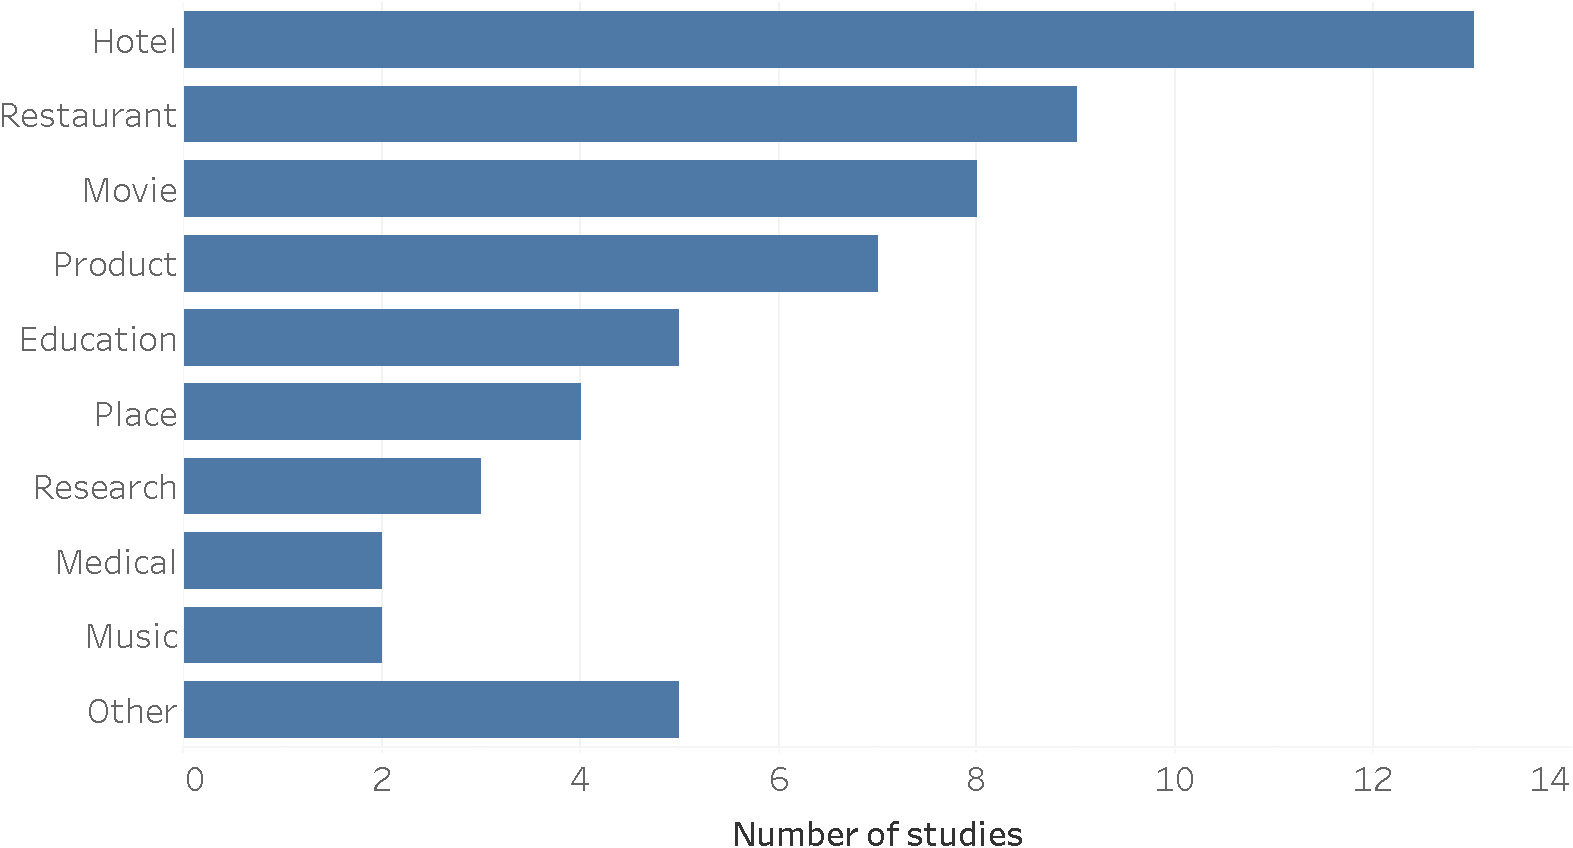
\includegraphics[width=\textwidth]{domain_per_study}
\caption[Studies per application domain]{This barplot represents the number of studies per application domain.}
\label{mcr:fig:domain-per-study}
\end{figure}

\subsection{Evaluation Protocols}
\label{mcr:sec:protocols}

In this section, we describe the evaluation protocols followed by the reviewed studies, in line with \ref{mcr:itm:rq6}. We grouped the possible evaluation strategies in four main categories, which are summarized in Table~\ref{mcr:tab:protocols}.

\subsubsection{Offline Comparison}

We discovered that 74 studies compare the proposed solution with other approaches using an offline evaluation. Multicriteria recommender systems are usually compared \added{against} traditional baselines such as single-criteria recommender or weighted average multicriteria approaches. Different studies consider the most similar methods already available in literature, while few studies only compare the described technique with itself, analyzing several configuration parameters.

\subsubsection{User Study}

A different approach is represented by the execution of user studies, which were carried out in 12 works. For example, the authors of \pref{slr:Akcayol2018} created a movie recommender system that was tested by 567 users. The researchers computed different metrics considering their behaviour while utilizing the recommender. In contrast, in \pref{slr:Li2015} 158 users were asked to fill out a questionnaire in order to compare different recommendation models. User studies are also exploited to evaluate the usability of the system, as done, for instance, in \pref{slr:Akhtarzada2011}.

\subsubsection{Case Study}

We also identified 4 studies that evaluated the proposed approach by describing a case study. For example, in \pref{slr:Hdioud2013}, a possible application of a multicriteria recommender to the movie domain is discussed, while the authors of \pref{slr:Lee2007} empirically compare the suggested restaurants considering different user profiles.

\subsubsection{No Evaluation}

Finally, 3 studies performed no evaluation of the multicriteria recommender presented in the paper. For example, in \pref{slr:Shambour2010}, the evaluation of the proposed model is left as a future work.

\begin{table}
\centering
\begin{tabular}{@{}ll@{}}
\toprule
Evaluation protocol & Studies \\ \midrule
Offline comparison  & 74      \\
User study          & 12      \\
Case study          & 4       \\
No evaluation       & 3       \\ \bottomrule
\end{tabular}
\caption[Studies per evaluation protocol]{The number of studies for each evaluation protocol.}
\label{mcr:tab:protocols}
\end{table}

\subsection{Evaluation Metrics}
\label{mcr:sec:metrics}

In the following, we discuss the metrics exploited in the reviewed studies for conducting the experimental evaluation of the proposed solutions in order to answer to \ref{mcr:itm:rq7}. We decided to classify them according to the dimensions related to the recommender system proprieties described by Gunawardana et al.~\cite{Gunawardana2015}. The identified category for each evaluation metric and the associated number of studies are reported in Table~\ref{mcr:tab:metrics}.

\subsubsection{Rating Accuracy}

This category includes metrics designed to evaluate the capability of the system to correctly estimate user ratings. In particular, 51 studies report the Mean Absolute Error (MAE), 20 the Root Mean Squared Error (RMSE), and 3 the Mean Squared Error (MSE). Other metrics exploited by 1 study each are the coefficient of determination ($R^2$) and the Mean Absolute Percentage Error (MAPE). In total, rating accuracy metrics are mentioned in 59 studies.

\subsubsection{Usage Accuracy}

If the goal of a recommender is to predict a list of items, it is possible to evaluate the usage accuracy of the available suggestions. Precision is considered in 36 studies, recall in 28, F1 in 23 studies, and Area Under the Curve (AUC) in 4 studies. Usage accuracy is the second most popular category, as it was identified in 43 studies.

\subsubsection{Coverage}

The metric of coverage was computed in 11 studies. Even if this metric can be evaluated both at the level of users and at the level of items, all the studies included in this review considered the coverage of the item space, also known as catalog coverage~\cite{Herlocker2004}.

\subsubsection{Ranking Accuracy}

The correctness of the ranking in the recommended lists of items was analyzed by 10 studies. In details, 8 studies exploit the Normalized Discounted Cumulative Gain (nDCG) metric, while 4 studies the Fraction of Concordant Pairs (FCP). A less popular metric, described by 1 study, is the Kendall's $\tau$.

\subsubsection{Scalability}

The authors of 8 studies evaluated the scalability of the proposed approach. A typical metric used to this purpose is the time required to compute the predictions, which is reported by 6 studies. In contrast, 2 studies exploit the speed of the recommendations.

\subsubsection{Other Metrics}

Additional metrics identified in the reviewed studies include the utility of the suggested items and the system satisfaction, evaluated with a user study, and the robustness of the recommendations. Finally, the authors of \pref{slr:Manouselis2014} defined a combined metric.

\begin{table}
\centering
\begin{tabular}{@{}ll@{}}
\toprule
Evaluation metric & Studies \\ \midrule
Rating accuracy   & 59      \\
Usage accuracy    & 43      \\
Coverage          & 11      \\
Ranking accuracy  & 10      \\
Scalability       & 8       \\
Other             & 5       \\ \bottomrule
\end{tabular}
\caption[Studies per evaluation metric]{The number of studies for each evaluation metric.}
\label{mcr:tab:metrics}
\end{table}

\subsection{Evaluation Datasets}
\label{mcr:sec:datasets}

In line with \ref{mcr:itm:rq8}, we analyzed the datasets exploited for conducting the experimental evaluation of the techniques described in the reviewed studies. In total, 74 studies mentioned at least one dataset: this result is consistent with the number of studies that performed an offline comparison, as reported in Section~\ref{mcr:sec:protocols}. We summarize the studies for each dataset in Figure~\ref{mcr:fig:dataset-per-study}.

\subsubsection{Yahoo! Movies}

Yahoo! Movies was a website, part of the Yahoo! network, that provided information and reviews about movies. Among other features, users were able to rate each movie considering five criteria: story, acting, direction, visuals, and overall. Yahoo! Research provides a public Yahoo! Movies dataset, but it does not include multicriteria ratings.\footnote{\url{https://webscope.sandbox.yahoo.com}} To address this issue, the authors of \pref{slr:Jannach2012} created a multicriteria version of the same dataset by crawling the Yahoo! Movies website. In total, 36 studies exploit the Yahoo! Movies dataset, either the version obtained by Jannach et al.~\pref{slr:Jannach2012} or other versions crawled by different researchers, \added{such as \pref{slr:Samatthiyadikun2013}, \pref{slr:Yin2009}, and \pref{slr:Adomavicius2007}.}

\subsubsection{TripAdvisor}

TripAdvisor is a website that contains restaurant and hotel reviews. Similarly to Yahoo! Movies, there is no official multicriteria rating dataset, as different researchers crawled the website and created their own version, typically exploiting hotel ratings and reviews. For example, this approach was followed by the authors of \pref{slr:Liu2010} and \pref{slr:Jannach2014}. The TripAdvisor dataset collected by the authors of \pref{slr:Liu2011} is publicly available.\footnote{\url{https://www.cs.cmu.edu/~jiweil/html/hotel-review.html}} Also the TripAdvisor dataset created by Wang et al.~\cite{Wang2010} and used in \pref{slr:Leal2017b} is available online.\footnote{\url{http://www.cs.virginia.edu/~hw5x/Data/LARA/TripAdvisor}} In total, the TripAdvisor dataset was mentioned by 19 studies.

\subsubsection{In-house}

We identified 9 studies that created a multicriteria dataset in-house for conducting an offline comparison. For example, the authors of \pref{slr:Palanivel2011} collected 9,628 ratings about songs that were later used to evaluate a music recommender system. In \pref{slr:Bokde2015}, different students were invited to provide ratings about universities.

\subsubsection{MovieLens}

Even if the MovieLens datasets only contain single criteria ratings, they were also exploited for evaluating multicriteria recommender systems. For instance, in \pref{slr:Shambour2011} \added{and in \pref{slr:Shambour2011b}}, MovieLens~100K was transformed in a four criteria dataset. A similar approach was followed in \pref{slr:Castillo2018} with MovieLens~10M, where a method capable of extracting multicriteria preferences from traditional ratings \added{using external aggregate ratings and descriptive data} is discussed. In total, the MovieLens datasets were mentioned by 5 studies.

\subsubsection{Synthetic}

Because of the lack of public multicriteria datasets, some researchers created synthetic ratings in order to evaluate their approach. For example, the authors of \pref{slr:Matsatsinis2009} simulated a dataset about equity fund recommendations. In \pref{slr:Manouselis2008}, a testing tool named CollaFiS, capable of building multicriteria datasets, is discussed. This approach was followed by 4 studies.

\subsubsection{Other Datasets}

Less common datasets, exploited by 1 or 2 studies each, include, for example, Bcn Restaurantes~\pref{slr:Marin2014}, HRS.com~\pref{slr:Leal2017b}, and RateBeer~\pref{slr:Ding2018b}. Such various datasets were considered by 18 studies.

\begin{figure}
\centering
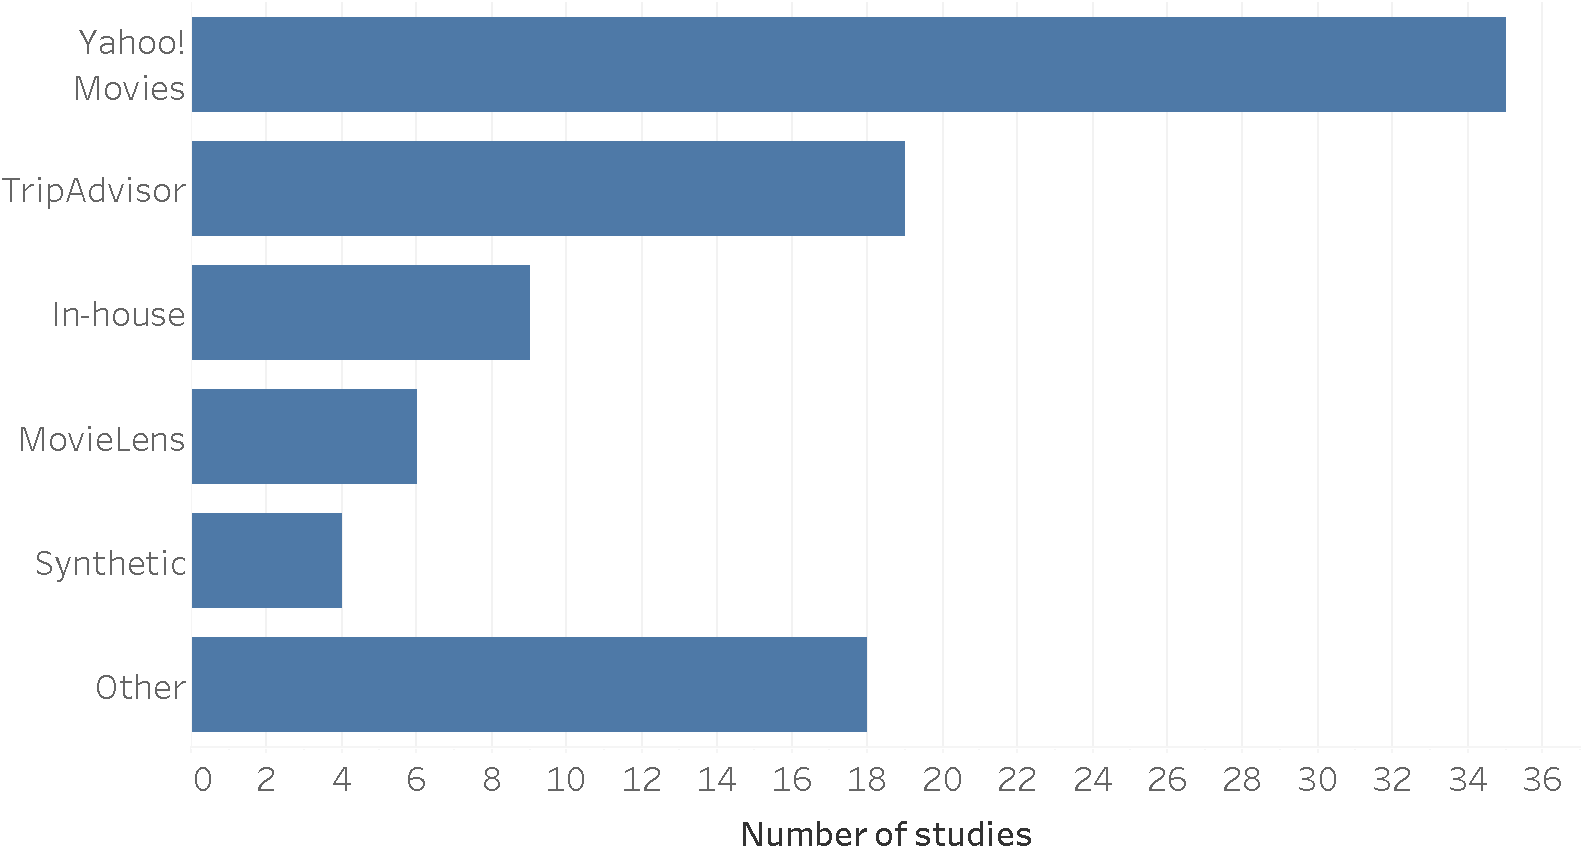
\includegraphics[width=\textwidth]{dataset_per_study}
\caption[Studies per evaluation dataset]{This barplot represents the number of studies per evaluation dataset.}
\label{mcr:fig:dataset-per-study}
\end{figure}

\subsection{Future Works}
\label{mcr:sec:future}

In the following, we analyze the suggestions for future works mentioned in the reviewed studies in order to provide an answer to \ref{mcr:itm:rq9}. A summary of our findings is available in Table~\ref{mcr:tab:future}.

\subsubsection{Extend the Solution}

Different authors propose to extend or modify the described recommender system for increasing its accuracy. \added{This future work is related to the problem of personalization, discussed in Section~\ref{mcr:sec:personalization}.} Common suggestions include adding additional components like clustering algorithms or further recommendation models and exploiting soft-computing techniques. In total, we identified this \added{future work} in 33 studies.

\subsubsection{Include More Data or Additional Criteria}

Another possibility is to improve the proposed approach by including more data or by increasing the number of criteria exploited by the recommendation algorithm. For example, it is possible to rely on external ontologies, contextual and content information, trust-related scores, and also consider additional criteria extracted from user reviews. This category of future works was mentioned in 24 studies.

\subsubsection{Improve the Evaluation}

Some studies mention the fact that the evaluation performed by their authors was not enough complete or detailed because of different kinds of constrains. For this reason, it would be advisable to increase its trustfulness by executing it again considering more datasets, techniques, and evaluation metrics. In total, this problem was reported by 14 studies.

\subsubsection{Identify Significant Criteria}

A common issue associated with multicriteria recommenders is the noise introduced by redundant criteria, \added{as discussed in Section~\ref{mcr:sec:data-noise}}. For this reason, some authors considered the identification of the most significant criteria as a future work. This suggestion was discussed in 13 studies.

\subsubsection{Increase the Scalability}

A typical issue of multicriteria recommender systems is their limited scalability. \added{This problem was highlighted by different studies in Section~\ref{mcr:sec:scalability}.} Some researchers suggested to study how to increase it, for example by means of parallel computational paradigms. We identified this future work in 10 studies.

\subsubsection{Consider Different Domains}

Finally, 7 studies mentioned the necessity of validating the proposed approach in different domains, like it is usually done with traditional recommenders. However, this objective is difficult to achieve because of the limited availability of multicriteria \added{rating} datasets.

\subsubsection{Other Future Works}

Further categories of future works, mentioned in less than 5 studies each, include designing solutions for addressing the cold-start problem, \added{as described in Section~\ref{mcr:sec:cold-start},} performing experiments with adaptive recommenders, solving the issues related to preference elicitation, creating algorithms for explaining the recommendations, and performing an analysis of the related ethical problems.

\begin{table}
\centering
\begin{tabular}{@{}ll@{}}
\toprule
Future work                   & Studies \\ \midrule
Extend the solution           & 33      \\
Include more data or criteria & 24      \\
Improve the evaluation        & 14      \\
Identify significant criteria & 13      \\
Increase the scalability      & 10      \\
Consider different domains    & 7       \\
Other                         & 9       \\ \bottomrule
\end{tabular}
\caption[Studies per category of future work]{The number of studies per category of future work.}
\label{mcr:tab:future}
\end{table}

\section{Discussion}
\label{mcr:sec:discussion}

In the following, we discuss the outcome of our systematic literature review, considering the answers provided in Section~\ref{mcr:sec:results} to the research questions originally introduced in Section~\ref{mcr:sec:questions}, and highlighting possible threats to validity.

\subsection{Included Studies}

As reported in Figure~\ref{mcr:fig:study-per-year}, the \added{earliest} study included in this review, which is \pref{slr:Karacapilidis2003}, dates back to the year 2003. However, the field of multicriteria recommender systems started to be relatively widespread only from the year 2007, when influential studies like \pref{slr:Adomavicius2007} were published. We can also observe an increasing amount of publications, suggesting that this research topic is still popular, as recommender systems in general. \added{In particular, the last few years were characterized by a higher number of studies related to specialized applications of multicriteria approaches, for example in tourism, health and care, and distance learning.}

Regarding the quality of the included studies, summarized in Figure~\ref{mcr:fig:quality-per-type}, we can highlight the fact that higher scores were assigned to works published in journals with respect to conferences. This result is consistent with the conclusions of other systematic literature reviews conducted in related fields, like hybrid and linked data-based recommender systems \cite{Cano2017,Figueroa2015}.

\subsection{Research Problems}

By looking at the problems listed in Section~\ref{mcr:sec:problems}, it is possible to observe that the most frequent one faced by researchers is data sparsity. This is a general issue of collaborative filtering recommender systems that causes a lower recommendation quality due to an insufficient amount of input data. However, it is reasonable to suppose that data sparsity is more severe in the context of multicriteria recommenders, because of the higher amount of expected ratings. Possible solutions include the use of external information or the construction of latent models. In contrast, it is not clear what is the effect of using different rating elicitation methods.

Another typical research problem is discovering what are the optimal weights for each criterion. They may be computed globally or for each user with the objective of maximizing the recommendation accuracy. A second approach is to obtain the weights directly from the user, for example with decision making techniques.

A different but related issue is represented by data noise, caused by redundant criteria or dishonest ratings. Of course, in order to minimize the user's effort and the probability of obtaining inaccurate ratings, it is necessary to limit the number of criteria. However, identifying the most appropriate ones for a given domain is a difficult task even for an expert. In our opinion, this issue should be better investigated by future studies.

Accuracy is a characteristic required for any machine learning technique and, in the context of recommender systems, it is related to user satisfaction. Multicriteria recommenders can increase the \added{personalization} of the suggestions if they are capable of correctly identifying what are the most important criteria for each user. However, when a user is new to the system, the cold-start problem arises. This is a general issue of collaborative filtering recommenders and it is typically solved by creating hybrid solutions that consider content-based information.

Finally, the usage of multiple \added{criterion} results in algorithms that are less scalable. This problem can be addressed with clustering and dimensionality reduction techniques, as well as by exploiting distributed architectures.

\subsection{Recommendation Approaches}

The vast majority of multicriteria recommender systems can be classified as collaborative filtering approaches, as reported in Table~\ref{mcr:tab:study-per-approach}. For example, in heuristic-based methods, the ratings provided for each dimension are exploited together using a multidimensional distance metric, extending the traditional neighborhood-based recommendation technique. More complex heuristics rely on the aggregation of different similarities computed per criterion, possibly using weights specific for each user. Also in the context of model-based collaborative filtering, methods like matrix factorization are applied to each dimension and, then, their results are aggregated in a global predicted rating.

For this reason, almost all recommender systems included in this review can be considered hybrid, as they combine multiple collaborative filtering models, one for each criterion. Furthermore, such techniques are sometimes exploited together with content-based, knowledge-based, community-based, and demographic approaches, resulting in other forms of hybrid recommenders~\cite{Burke2007}.

However, a limited number of studies included in this review deals with recommender systems that can be classified only as knowledge-based. Such systems exploit domain specific knowledge to match the available items with the user preferences. They were selected because we identified them as a form of multicriteria recommendation, even if the distinction between knowledge-based recommenders and traditional information retrieval methods is not always clear.

\subsection{Multicriteria Techniques}

In Section~\ref{mcr:sec:techniques}, we reported that the most common technique exploited by multicriteria recommenders is the \textit{k}-NN algorithm. This result is consistent with the recommendation approaches identified in the reviewed studies, as neighborhood-based methods represent a popular approach of collaborative filtering. \textit{k}-NN may be enough to build a multicriteria recommender: the similarities among users or items can be directly computed with a multidimensional distance metric and they can be aggregated using a trivial approach, like the averaging function, or estimated by means of more complex techniques.

In contrast, multicriteria matrix manipulation methods represent a less common approach to collaborative filtering and they are often exploited to estimate unknown ratings for each criterion or to reduce the dimensionality of the problem. Again, matrix manipulation methods are usually combined with other methods designed to estimate importance weights for each criterion.

Different families of such techniques have been identified in the reviewed studies namely, regression analysis, neural networks, and genetic algorithms. It is possible to produce an overall rating using regression analysis if the other methods are not capable of dealing with multiple ratings on their own. A more recent alternative to regression analysis is represented by neural networks, that are exploited for learning the relative importance of criteria. Finally, genetic algorithms may be used to discover the weights of each criterion, but also to estimate good parameters for the recommendation model.

For reducing the complexity of the problem, some studies considered clustering algorithms in order to create cohesive groups of similar users or items. Such algorithms are usually applied as a first step, before other techniques capable of creating suggestions suitable for each cluster. In contrast, fuzzy logic may be exploited together with all the aforementioned methods for formally encoding the fact that ratings usually represent uncertain values.

The second most popular recommendation method after \textit{k}-NN consists in decision analysis techniques. They are typically used to generate an ordered list of suggested items considering potential conflicts in user requirements. Decision analysis algorithms are often combined with \textit{k}-NN, matrix manipulation, and clustering methods. However, some studies do not mention a specific recommendation technique to be exploited jointly with a decision analysis method because the proposed approach is presented as a general framework and, thus, any recommendation method is suitable.

In Table~\ref{mcr:tab:comparison}, we report the main benefits and issues of the reviewed multicriteria methods. They could be considered as different compromises between the correctness of the suggestions and the complexity of the approach. Thus, it is of paramount importance being able to decide if, for a given task, it is more appropriate to foster the scalability of the system or the accuracy of the results.

\begin{sidewaystable}[p]
\begin{tabularx}{\linewidth}{lXX}
\toprule
Technique & Benefit & Issue \\ \midrule
\textit{k}-NN & It can compute directly the predictions using a multidimensional metric. & If it is combined with other methods its scalability is reduced. \\
Decision analysis & It can analyze the importance that each user gives to the available criteria. & It may require additional data from the users apart their multicriteria ratings. \\
Fuzzy logic & It supposes that rating values may have a different meaning depending on the user. & It must be combined with additional techniques to actually recommend items. \\
Regression analysis & It is the most popular approach for discovering the individual weight of each criteria. & It must be combined with \textit{k}-NN or matrix manipulation. \\
Clustering & It can create groups of users with similar rating behaviours and reduce the dimension of the problem inputs. & It must be exploited together with additional techniques. \\
Matrix manipulation & It can compute unknown ratings for each criteria in an efficient and effective way. & It usually require a final step to calculate an overall predicted rating. \\
Neural network & Recent approaches can directly predict the final ratings with an interesting accuracy. & It is often exploited to compute the weights of each criteria, adding more complexity. \\
Generic algorithm & It can automatically determine the optimal weight for each criteria and user. & It must be combined with additional techniques to predict the final ratings. \\ \bottomrule
\end{tabularx}
\caption[Benefits and issues of the techniques]{The main benefits and issues of the reviewed techniques.}
\label{mcr:tab:comparison}
\end{sidewaystable}

Finally, in Figure~\ref{mcr:fig:techniques}, we summarize how such techniques could be exploited for constructing an ideal multicriteria recommender. In the preprocessing phase, common approaches designed to reduce the dimension of the input ratings are clustering and genetic algorithms. Also fuzzy logic may be applied at this point to transform the ratings in fuzzy numbers. During the rating prediction phase, it is possible to rely on \textit{k}-NN, matrix manipulation methods, neural networks, and statistical models. These algorithms may already include a dimensionality reduction step and a way of obtaining an ordered list of suggestions. Finally, in the ranking phase, popular approaches are decision analysis, regression analysis, neural networks, and genetic algorithms. Please note that the first and third phase are, in general, optional and they add several layers of complexity to the developed system. Furthermore, some techniques may already perform these tasks during the rating prediction phase.

\begin{figure}
\centering
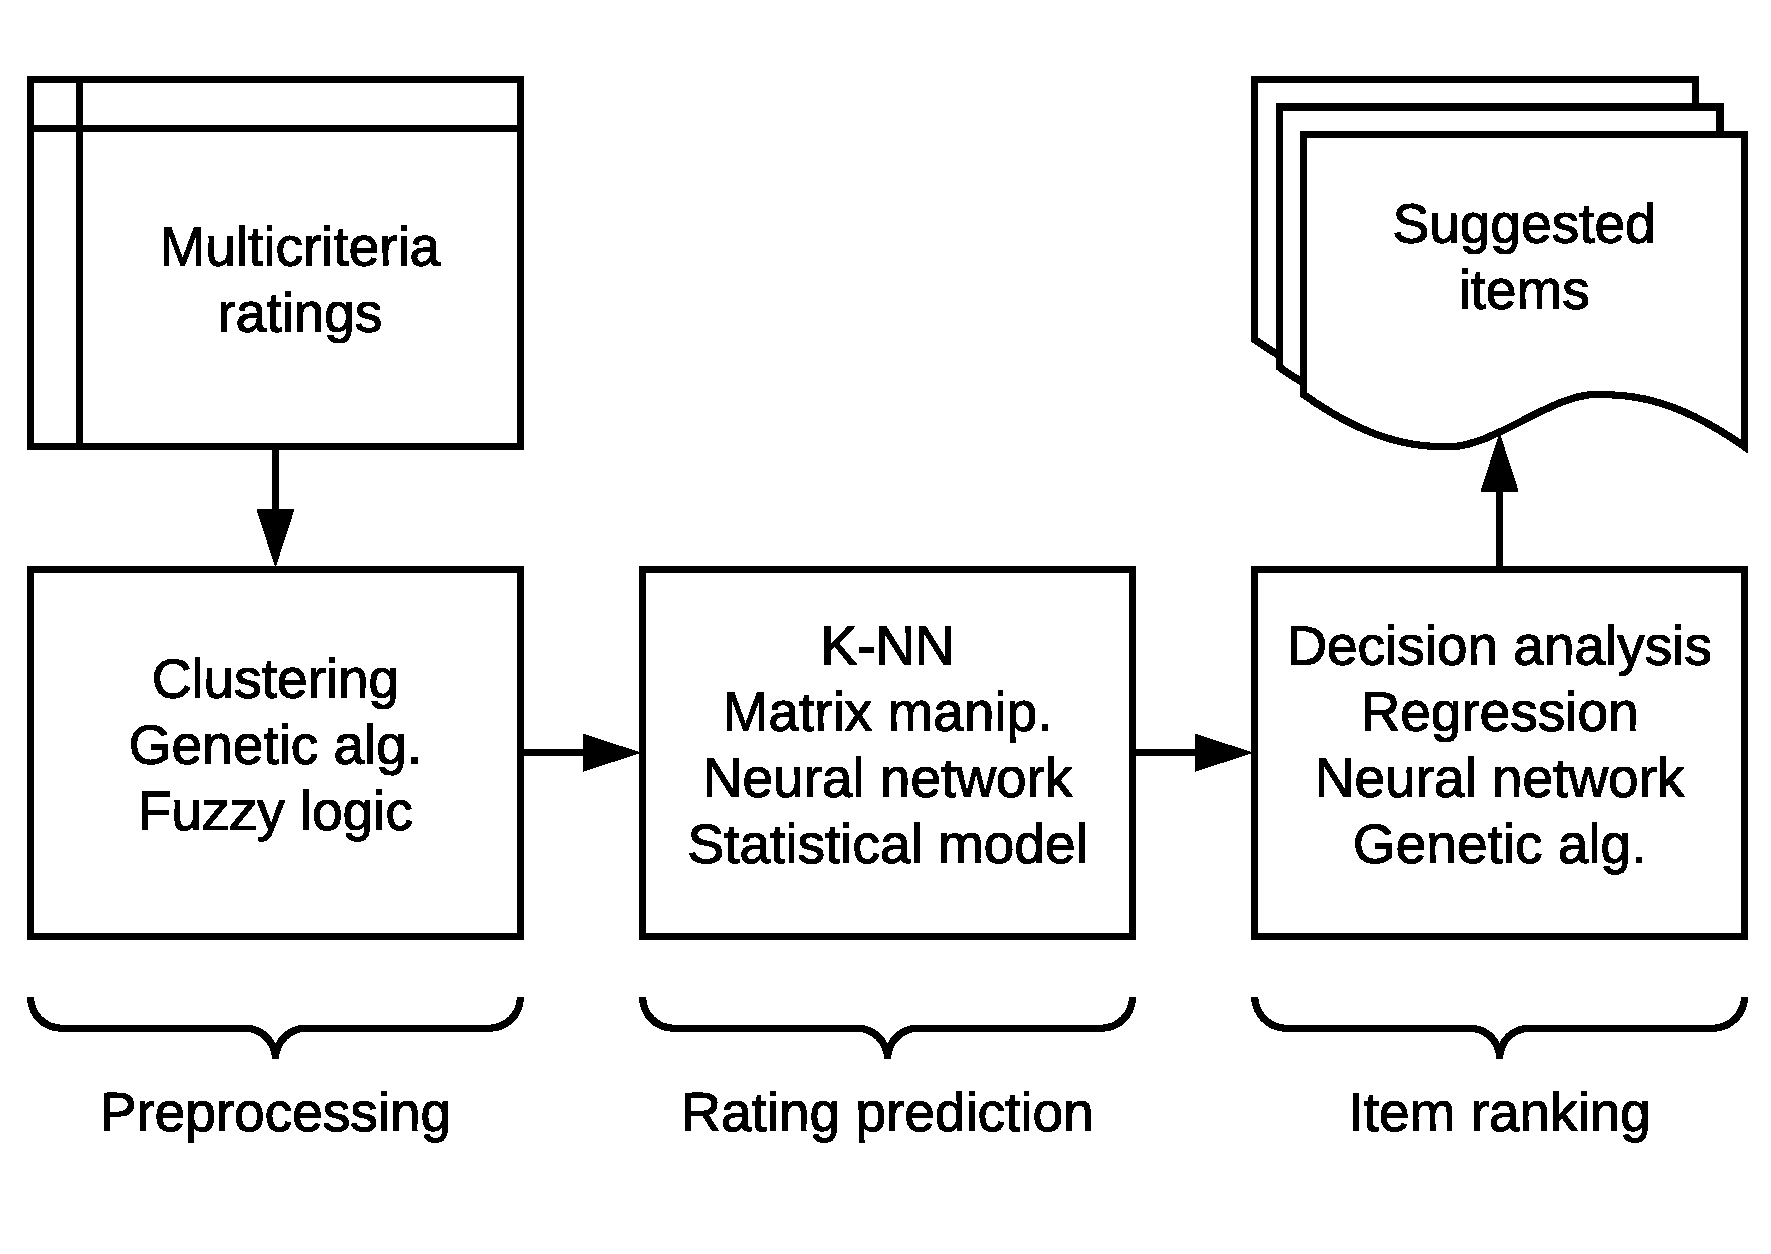
\includegraphics[width=.9\textwidth]{multicriteria_techniques}
\caption[Ideal multicriteria recommender]{This diagram represents the possible techniques exploited by an ideal multicriteria recommender, subdivided according to the recommendation phase. Content-based features and other less common approaches are not considered.}
\label{mcr:fig:techniques}
\end{figure}

\subsection{Application Domains}

As already observed in Section~\ref{mcr:sec:domains}, multicriteria recommenders are frequently exploited in the tourism and travel domain. This result is \added{expected}, as many travel websites, like TripAdvisor\footnote{\url{https://www.tripadvisor.com}} and Bcn Restaurantes,\footnote{\url{https://www.bcnrestaurantes.com}} rely on multicriteria ratings for suggesting items to their users. Even for someone that is not a domain expert, it is possible to identify some useful criteria that should be considered when evaluating a hotel or a restaurant.

For this reason, we can suppose that items belonging to complex domains can be more easily analyzed considering different dimensions and, therefore, they are better suited for multicriteria recommender systems. Another popular example is represented by consumer products, which can be evaluated considering different criteria based on their features, price, and quality.

On the other hand, domains like music or books are usually not exploited for creating a multicriteria recommender, probably because assigning detailed evaluations of such items is too difficult for someone that is not a domain expert.

Another factor that must be considered before performing further analysis is the availability of a certain multicriteria rating dataset in a particular domain. For example, many researchers used to collected ratings from the Yahoo! Movies website, but nowadays such service is no longer available.

The majority of the recommender systems presented in the reviewed studies are domain-independent, as they are only based on multicriteria ratings. However, some solutions designed for specific domains, like medical treatments and research papers, cannot be easily adapted to other scenarios.

\subsection{Evaluation Protocols}

In general, performing the evaluation of a recommender system is a complex task, because the slightest change in the experimental protocol may produce radically different results~\cite{Said2014}. It is not possible to directly compare the outcomes of different works because of the great variety of datasets, evaluation protocols, and metrics mentioned in the reviewed studies.

The multicriteria recommender systems were often evaluated using offline comparisons, as summarized in Table~\ref{mcr:tab:protocols}. This result is \added{expected}, as such \added{an} approach is less expensive \added{than} performing a user study, but it can be used to obtain useful information. However, in order to report more conclusive results, some authors decided to perform a user study. We noticed that it is difficult to involve a significant number of experimental subjects. In fact, only in 3 studies the number of participants was higher than a hundred people.

\subsection{Evaluation Metrics}

The majority of the reviewed studies validated their approach using \added{rating} accuracy metrics, as reported in Table~\ref{mcr:tab:metrics}. This result is probably related to the fact that recommender systems were initially considered as tools designed to predict unknown ratings as accurately as possible. This evaluation approach produces results that are interesting from an academic point of view, but they may have a limited practical meaning.

In fact, as suggested in \cite{Herlocker2000}, it is not possible to display in an application all the items that are associated with the highest predicted ratings. Therefore, it is necessary to be capable of correctly creating lists of ranked items that will be shown to users. This aspect is considered by different studies, in which usage and ranking accuracy metrics are reported.

Other categories of metrics identified during the review include coverage and scalability, which were evaluated in a relatively low number of studies. It is interesting to notice that more recent evaluation dimensions, like diversity, novelty and serendipity, have not been considered, suggesting that their adoption in the recommender system community is still limited.

Finally, we also observed that the differences in the evaluation protocols followed by the reviewed studies do not allow a direct comparison of the results, even when widespread metrics, like MAE or precision, are exploited. \added{For example, we identified a wide variability in the rating dataset, the splitting method between training and test set, and the definition of non-relevant items.} This conclusion is consistent with the findings reported in \cite{Said2014}.

\subsection{Evaluation Datasets}

From the results presented in Section~\ref{mcr:sec:datasets}, we observe that different evaluation datasets have been created using data available in online portals that contain multicriteria ratings. Such collections of ratings are usually not directly provided by the platforms, like the MovieLens datasets, but they are downloaded by researchers using web crawling methods. These approaches result in different versions of the same dataset that sometimes are not publicly available and they can only be obtained by contacting the original creators.

Consider, for example, Yahoo! Movies: this dataset was realized by adding multicriteria ratings to a collection of movie preferences initially provided by Yahoo! Research, quickly becoming one of the most widespread multicriteria gold standards. However, the Yahoo! Movies platform does not provide multicriteria ratings anymore, making impossible to recreate it. Similar observations are also valid for other datasets, as platforms may change over the years and original datasets may become unavailable. \added{Anyway}, we were able to locate two TripAdvisor dataset versions that are still publicly available on the Web.

It is interesting to notice that the authors of different studies decided to create new datasets, relying on real users and simulation tools, or to add additional criteria to existing datasets. This fact suggests that there is the need of realizing and publishing further multicriteria datasets.

\subsection{Future Works}

We described the main future work directions reported by the authors of the reviewed studies in Section~\ref{mcr:sec:future}, in order to identify how it is possible to advance the multicriteria recommender field. The most common suggestion is to add to the proposed technique an additional component for improving its \added{personalization}. The authors of such recommenders usually observe that their methods could benefit from further preprocessing phases or additional components to be combined in a hybrid approach. Another possibility is to consider soft-computing techniques for expressing the uncertainty and vagueness of user ratings.

It is interesting to notice that some studies propose to improve multicriteria recommenders by considering further data, while other authors are more interested in reducing the number of available criteria. These suggestions are not in contrast, as they may be related to the exploited dataset. Therefore, correctly defining the rating criteria and better studying how such ratings are collected are of paramount importance for obtaining high quality recommendations.

Different works propose to also consider friendship relations among users, external knowledge bases and ontologies, and more contextual information. Social Recommender Systems (SRS)~\cite{Guy2015}, Semantics-Aware Recommender Systems (SARS)~\cite{Gemmis2015a}, and Context-Aware Recommender Systems (CARS)~\cite{Adomavicius2015a} are relatively new recommendation approaches that could be exploited jointly with multicriteria techniques in order to create a more personalized experience. However, such additional data need to be managed in a proper way: for this reason, some researchers propose to also study the scalability of the available solutions.

As already discussed, recommender system evaluation is not an easy task. Therefore, different authors declare that they plan to conduct a more extensive experimentation of the proposed approach in future works. This frequent situation may be caused by the difficulties in obtaining multicriteria datasets or by the elevated costs necessary for involving real users in the evaluation process. A related future work is to evaluate the same approach in different domains, as also this suggestion requires further datasets and experiments.

\subsection{Threats to Validity}

In this section, we point out the main problems that we addressed while conducting this systematic literature review. We noticed that there is no strong agreement on a shared definition of multicriteria recommender systems, as there are some subtle differences but also some similarities with multiattribute content-filtering techniques~\cite{Adomavicius2015}. For this reason, we only considered as multicriteria the recommenders based on multicriteria ratings. We also included in our selection few studies describing methods that cannot be considered collaborative filtering approaches, but that exploit multicriteria ratings in a non-conventional way. Furthermore, a limited number of studies were initially selected by analyzing their title and abstract. However, we were later forced to exclude them even if they were potentially relevant because we were not able to retrieve their full-text version. We also noticed that some studies were described in different research papers, and, therefore, we analyzed these situations with attention. Sometimes we selected multiple works because we discovered that these contributions were only partially overlapped.

\section{Conclusion}
\label{mcr:sec:conclusions}

In the context of this systematic literature review, we analyzed a total number of 93 studies related to the topic of multicriteria recommender systems. We provided an answer to nine different research questions, in order to identify which are the main problems that multicriteria recommenders aim to resolve, what recommendation approaches they usually exploit, and what are the most common machine learning and data mining techniques considered for realizing them. Furthermore, we investigated in which domains multicriteria recommenders can be applied, how they are evaluated in terms of experimental protocols, metrics, and rating datasets. Finally, we reported the most common suggestions available in selected studies for conducting future research works.

We identified data sparsity as the most frequent problem that researchers try to address. This issue could be caused by the fact that users are less willing to provide multicriteria ratings because they find this task difficult and time consuming, as they need to consider different aspects of the same item separately. A related research problem is understating what are the most appropriate criteria that should be considered in a particular domain. An excessive number of criteria will most likely result in a partial overlap of their meanings, thus causing a reduction of the prediction accuracy because of the additional noise in the input data. Further studies should better quantify what is the impact of this problem and how recommendation algorithms could reduce it.

We observed that almost all multicriteria recommenders rely on collaborative filtering techniques. This approach is, in fact, also popular in the context of single-criteria recommenders. A large portion of the reviewed studies propose hybrid recommendation methodologies, as they usually combine multiple runs of collaborative filtering algorithms, one for each criterion. However, we also observed a more recent trend of also relying on additional techniques, like content-based, knowledge-based, and community-based approaches. The motivating idea of such recommender systems is to increase the accuracy of the suggested items by exploiting further data behind pure multicriteria ratings.

Furthermore, we classified the machine learning and data mining techniques mentioned in the reviewed studies according to the recommendation phase in which they are considered. We observed that during the preprocessing phase different authors choose to reduce the dimension of the problem inputs by means of clustering and genetic algorithms. In the rating prediction phase, various collaborative filtering methods are considered, like \textit{k}-NN, matrix manipulation techniques, neural networks, and statistical models. Finally, during the ranking phase, it is possible to rely on decision analysis, regression analysis, neural networks, and genetic algorithms. Such methods are combined in various ways, and sometimes integrated with the results of additional recommendation approaches.

We also investigated the domains that are usually considered for implementing a multicriteria recommender system. In the reviewed studies we frequently observed items related to the tourism and travel domain, for example hotels and restaurants. Another popular domain is represented by movies, probably due to the past availability of the Yahoo! Movies datasets. In contrast, domains that are often exploited in single-criteria recommenders, like music or books, are almost never considered for multicriteria approaches. Possible explanations of this finding could be the lack of proper evaluation datasets or the difficulties in defining meaningful criteria and obtaining the associated ratings.

From the analyzed experiments we observed that \added{it} is not possible to directly compare the results obtained with different recommendation approaches due to the extreme variability in the experimental protocols followed by their authors. Another critical point that emerged from this work is the lack of publicly available multicriteria rating datasets. Even if this problem could be partially mitigated with synthetic and crawled datasets, additional efforts should be done in order to \added{create} proper benchmarks in different domains and, thus, enabling a better reproducibility of the experimental results.

Finally, our findings indicate that future works in this field should better explore how to increase the utility of multicriteria recommenders by integrating community-based, knowledge-based, and context-aware approaches, according to the peculiar characteristics of the recommended items. For example, a restaurant recommender system would greatly benefit from context-aware information, a movie recommender could also leverage on semantic data, while a consumer product recommender may assign more importance to the opinions of trusted users. Another interesting point that should be better addressed in future works is defining what are the most appropriate criteria for each domain and how the ratings associated to that criteria should be collected in order to minimize user efforts, also considering soft-computing and linguistic techniques. Furthermore, it would be useful to explore novel algorithms for dynamically understanding the importance that each user implicitly assigns to a criterion, for reducing the fatigue associated with the preference elicitation phase.
